\section{质点运动学}

\subsection{位移、速度、加速度}

\begin{enumerate}
	\item 位置矢量（位矢）
	\begin{itemize}
		\item 建立直角坐标系后，物体的位置可用坐标 $A(x,y,z)$ 表示。
		\item 向量 $\vec{r}=\overrightarrow{OA}$ 就称为位置矢量（位矢），也记为
		\begin{align*}
			\vec{r}=x\vec{i}+y\vec{j}+z\vec{k}.
		\end{align*}
	\end{itemize}
	
	\item 运动方程
	\begin{itemize}
		\item 质点坐标 $x,y,z$ 随 $t$ 的变化关系，将 $t$ 消掉即可。
	\end{itemize}

	\item 位移与路程
	\begin{itemize}
		\item 物体的位置变化称为位移 $\Delta \vec{r}$，用起点到终点的有向线段表示。
		\item 物体实际运动的路径长称为路程 $\Delta s$。
		\item \textcolor{red}{注意}
		\begin{itemize}
			\item $\Delta \vec{r}$ 是位移，$\lvert \Delta \vec{r} \rvert$ 是位移的大小，$\Delta r$ 是物体到原点距离的变化。
			\item 只有 $ds=\lvert d\vec{r} \rvert$ 是对的，$\Delta s \neq \lvert \Delta \vec{r} \rvert$，$\lvert \Delta \vec{r} \rvert \neq \Delta r$，$\lvert d\vec{r} \rvert \neq dr$。
			\item 出现 $\Delta r$、$dr$ 基本都是错的。
		\end{itemize}
	\end{itemize}
	
	\item 速度与速率
	\begin{itemize}
		\item 平均速度为位移除以时间，平均速率是路程除以时间：
		\begin{align*}
			\vec{v}=\frac{\Delta \vec{r}}{\Delta t}, 
			\qquad
			\bar{v}=\frac{\Delta s}{\Delta t}.
		\end{align*}
		
		\item 瞬时速度就是对每个坐标分量求导：
		\begin{align*}
			\vec{v}
			=\frac{d\vec{r}}{dt}
			=\frac{dx}{dt}\vec{i}
			+\frac{dy}{dt}\vec{j}
			+\frac{dz}{dt}\vec{k}.
		\end{align*}
		
		\item 瞬时速率是瞬时速度的大小：
		\begin{align*}
			v
			=\left|\frac{d\vec{r}}{dt}\right|
			=\frac{ds}{dt}
			=\sqrt{
				\left(\frac{dx}{dt}\right)^2
				+\left(\frac{dy}{dt}\right)^2
				+\left(\frac{dz}{dt}\right)^2
			}.
		\end{align*}
		
		\item \textbf{注意：}不能写成
		\begin{align*}
			\frac{dr}{dt}
			\quad \text{或} \quad
			\frac{d|\vec{r}|}{dt}.
		\end{align*}
	\end{itemize}

	\item 加速度
	
	\begin{itemize}
		\item 平均加速度
		\begin{align*}
			\vec{a} = \frac{\Delta \vec{v}}{\Delta t}
		\end{align*}
		
		\item 瞬时加速度就是对每个速度分量求导
		\begin{align*}
			\vec{a}
			= \frac{d\vec{v}}{dt}
			= \frac{dv_x}{dt}\vec{i}
			+ \frac{dv_y}{dt}\vec{j}
			+ \frac{dv_z}{dt}\vec{k}
		\end{align*}
		
		\item \textbf{注意：}加速度与速度同号为加速，异号为减速，而不是正数加速、负数减速。
	\end{itemize}
	
	
	\item 位移、速度、加速度的互求
	
	\begin{align*}
		v &= \frac{dx}{dt}, \qquad
		a = \frac{dv}{dt}, \qquad
		v = v_0 + \int_0^t a\,dt, \qquad
		x = x_0 + \int_0^t v\,dt
	\end{align*}
	
\end{enumerate}

\newpage

\subsection{例题1}

\begin{enumerate}

\item 已知质点的运动学方程为
\begin{align*}
	\vec{r}=4t^{2}\vec{i}+(2t+3)\vec{j},
\end{align*}

则质点的运动方程为\underline{\hspace{4cm}}。


\item 一运动质点在某瞬时位于矢径 $\vec{r}=(x,y)$ 的端点处，其速度大小为(\quad).

\begin{choices}
	\item $\dfrac{dr}{dt}$
	\item $\dfrac{d\vec{r}}{dt}$
	\item $\dfrac{d|\vec{r}|}{dt}$
	\item $\sqrt{\left(\dfrac{dx}{dt}\right)^2+\left(\dfrac{dy}{dt}\right)^2}$
\end{choices}

\item 一质点在 $Oxy$ 平面内运动。运动学方程为
\begin{align*}
	x=2t,\qquad y=19-2t^2,
\end{align*}

则在第 $2$ 秒内质点的平均速度大小为\underline{\hspace{1.5cm}}，第 $2$ 秒末的瞬时速度大小为\underline{\hspace{1.5cm}}。


\item 某质点作直线运动的运动学方程为
\begin{align*}
	x = 3t - 5t^3 + 6
\end{align*}

则该质点作

\begin{enumerate}
	\item[A.] 匀加速直线运动，加速度沿 $x$ 轴正方向
	\item[B.] 匀加速直线运动，加速度沿 $x$ 轴负方向
	\item[C.] 变加速直线运动，加速度沿 $x$ 轴正方向
	\item[D.] 变加速直线运动，加速度沿 $x$ 轴负方向
\end{enumerate}

\item 一质点沿 $x$ 方向运动，其加速度随时间变化关系为$a = 3 + 2t$，如果质点从原点出发，初始时的速度 $v_0$ 为$5\,\mathrm{m/s}$，则当 $t$ 为 $3\,\mathrm{s}$ 时，质点的速度$v = \underline{\hspace{3cm}}$，位置坐标为$x = \underline{\hspace{3cm}}$。


\end{enumerate}

\newpage
\subsection{圆周运动的参数}

\begin{enumerate}
	
	\item 切向与法向加速度
	
	\begin{itemize}
		\item 加速度可以沿速度方向分解。
		
		\item 与速度方向平行的称为切向加速度，改变速度的大小：
		\begin{align*}
			a_t = \frac{dv}{dt}
		\end{align*}
		
		\item 与速度方向垂直的称为法向加速度，改变速度的方向：
		\begin{align*}
			a_n = \frac{v^2}{\rho}
		\end{align*}
		
		\item 其中 $\rho$ 为曲率半径，若为圆周运动就为半径。
	\end{itemize}
	
	\item 圆周运动参数的互求
	
	\begin{align*}
		\omega &= \frac{d\theta}{dt}, \qquad
		\alpha = \frac{d\omega}{dt}, \qquad
		\omega = \omega_0 + \int_{0}^{t} \alpha \, dt, \qquad
		\theta = \theta_0 + \int_{0}^{t} \omega \, dt
	\end{align*}
	
	\item 角量与线量的关系
	
	\begin{itemize}
		\item 线速度
		\begin{align*}
			v = \omega R
		\end{align*}
		
		\item 法向加速度
		\begin{align*}
			a_n = \frac{v^2}{R} = \omega^2 R
		\end{align*}
		
		\item 切向加速度
		\begin{align*}
			a_t = \frac{dv}{dt} = \alpha R
		\end{align*}
	\end{itemize}
	
	
	
	
\end{enumerate}

\newpage
\subsection{例题2}

\begin{enumerate}
	
	\item 在半径为 $R$ 的圆周上运动的质点，其速率与时间关系为 $v = ct^2$，从 $0$ 时刻到 $t$ 时刻，质点走过的路程为 $s = \underline{\hspace{3cm}}$；$t$ 时刻质点的切向加速度为 $a_t = \underline{\hspace{2.5cm}}$，法向加速度为 $a_n = \underline{\hspace{2.5cm}}$，总加速度的大小为 $a = \underline{\hspace{2.5cm}}$。
	
	\item 一质点从静止出发，沿半径为 $R=1$ 的圆周运动，角加速度
	$\alpha = 12t^2 - 6t$，则质点的角速度
	$\omega = \underline{\hspace{2cm}}$，切向加速度
	$a_t = \underline{\hspace{2cm}}$，法向加速度
	$a_n = \underline{\hspace{2cm}}$，总加速度为
	$a = \underline{\hspace{2cm}}$。
	
\end{enumerate}


\newpage
\section{质点动力学}

\subsection{牛顿运动定律}

\begin{enumerate}
	\item \textbf{牛顿第一定律：}任何物体都保持静止或匀速直线运动的状态，除非作用在它上面的力迫使它改变这种状态。
	
	\item \textbf{牛顿第二定律：}$\vec{F}=\frac{d\vec{p}}{dt}$，若质量不变，则$\vec{F}=m\frac{d\vec{v}}{dt}=m\vec{a}$。
	
	\item \textbf{牛顿第三定律：}$\overrightarrow{F}_{12}=-\overrightarrow{F}_{21}$。
\end{enumerate}

\newpage
\subsection{例题1}

\begin{enumerate}
	\item 质量为 \(m\) 的物体系于长度为 \(R\) 的绳子的一个端点上，在竖直平面内绕绳子另一端点（固定）作圆周运动。设 \(t\) 时刻物体瞬时速度的大小为 \(v\)，绳子与竖直向上的方向成 \(\theta\) 角。求 \(t\) 时刻绳中的张力 \(T\) 和物体的切向加速度 \(a_t\)。

	\begin{figure}[H]
		\centering
		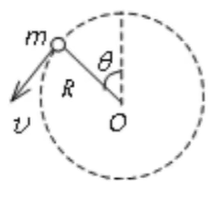
\includegraphics[width=0.15\linewidth]{figures/screenshot001}
		%\caption{}
		\label{fig:screenshot001}
	\end{figure}
	
	\item 质量为 \(m\) 的子弹以速度 \(v_0\) 水平射入沙土中，设子弹所受阻力与速度反向，大小为 \(f=Kv\)（\(K\) 为比例系数），忽略子弹的重力，求：
	\begin{enumerate}
		\item 子弹射入沙土后，速度随时间变化的函数式；
		\item 子弹进入沙土的最大深度。
	\end{enumerate}
	
	
\end{enumerate}

\newpage
\subsection{动量定理}

\begin{enumerate}
	\item 冲量：
	\begin{align*}
		\vec{I}=\int_{t_1}^{t_2}\vec{F}\,dt
	\end{align*}
	动量：
	\begin{align*}
		\vec{p}=m\vec{v}
	\end{align*}
	
	\item 质点动量定理：
	\begin{align*}
		\vec{I}=\int_{t_1}^{t_2}\vec{F}\,dt=\vec{p}_2-\vec{p}_1
		\quad \text{或} \quad
		\vec{F}\,dt=d\vec{p}
	\end{align*}
	
	\begin{itemize}
		\item 要想求平均冲力，即假设 $\vec{F}$ 不变，有
		\begin{align*}
			\vec{F}\Delta t=\Delta \vec{p}=m\vec{v}_2-m\vec{v}_1
		\end{align*}
	\end{itemize}
	
	\item 质点系动量定理：
	\begin{align*}
		\vec{I}=\int_{t_1}^{t_2}\vec{F}_{\text{外}}\,dt=\vec{p}_2-\vec{p}_1
		\quad \text{或} \quad
		\vec{F}_{\text{外}}\,dt=d\vec{p}
	\end{align*}
	
	\begin{itemize}
		\item 注意质点系动量定理与内力无关
	\end{itemize}
	
	\item 动量守恒定律
	
	\begin{itemize}
		\item 原点系所受合外力为零时，总动量不变
		\begin{itemize}
			\item 动量守恒的条件是质点系的合外力为零
			\item 若系统在某个方向上的合外力为零，则在该方向上动量守恒
			\item 对于碰撞、爆炸问题，可近似认为动量守恒
		\end{itemize}
	\end{itemize}
	
	
\end{enumerate}

\newpage
\subsection{例题2}

\begin{enumerate}
	\item 如图所示，砂子从 $h=0.8\,\mathrm{m}$ 高处下落到以 $3\,\mathrm{m/s}$ 的速率水平向右运动的传送带上。传送带给刚落到传送带上的砂子的作用力的方向为(\quad).
	
	\begin{figure}[H]
		\centering
		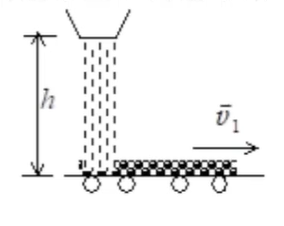
\includegraphics[width=0.25\linewidth]{figures/screenshot004}
		%\caption{}
		\label{fig:screenshot004}
	\end{figure}
	
	\begin{choices}
		\item 与水平夹角 $53^\circ$ 向下
		\item 与水平夹角 $53^\circ$ 向上
		\item 与水平夹角 $37^\circ$ 向上
		\item 与水平夹角 $37^\circ$ 向下
	\end{choices}
	
	\item 一吊车底板上放一质量为 $10\,\mathrm{kg}$ 的物体，若吊车底板加速上升，加速度大小为 $a=3+5t$，则 $2$ 秒内物体动量的增量大小为\underline{\hspace{4cm}}；$2$ 秒内吊车底板给物体的冲量大小为\underline{\hspace{4cm}}。
	
	\item 有两个长方形的物体 A 和 B 紧靠着静止放在光滑的水平桌面上，已知 $m_A=2\,\mathrm{kg}$，$m_B=3\,\mathrm{kg}$。现有一质量 $m=100\,\mathrm{g}$ 的子弹以速率 $v_0=800\,\mathrm{m/s}$ 水平射入长方体 A，经 $t=0.01\,\mathrm{s}$，又射入长方体 B，最后停留在长方体 B 内未射出。设子弹射入 A 时所受的摩擦力为 $F=3\times10^3\,\mathrm{N}$，求：
	
	\begin{figure}[H]
		\centering
		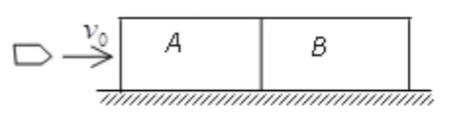
\includegraphics[width=0.35\linewidth]{figures/screenshot002}
		%\caption{}
		\label{fig:screenshot002}
	\end{figure}
	
	\begin{enumerate}
		\item 子弹在射入 A 的过程中，B 受到 A 的作用力的大小。
		\item 当子弹留在 B 中时，A 和 B 的速度大小。
	\end{enumerate}
	
	\item 质量为 \(m\) 的小物体从质量为 \(M\) 的斜面顶端下滑，斜面长度为 \(L\)，倾斜角为 \(\theta\)，假设各接触面均光滑，求物体滑到底端时，斜面的位移。
	
\end{enumerate}

\newpage
\subsection{角动量守恒定律}

\begin{enumerate}
	\item 角动量
	\begin{itemize}
		\item 质点对固定的点 $O$ 的角动量为 $\vec{L}=\vec{r}\times\vec{p}=m\vec{r}\times\vec{v}$
		\item 匀速圆周运动的质点对圆心的角动量是 $L=mvR$
	\end{itemize}
	
	\item 力矩：$\vec{M}=\vec{r}\times\vec{F}$
	
	\item 角动量定理：$\displaystyle \int_{t_1}^{t_2}\vec{M}\,dt=\vec{L}_2-\vec{L}_1$ 或 $\vec{M}\,dt=d\vec{L}$
	
	\item 角动量守恒定律
	\begin{itemize}
		\item 若力矩为零，则角动量不变
		\item 如果合外力为 $0$，则力矩当然为 $0$，角动量守恒
		\item 如果外力始终过定点，则相对于这个点，角动量守恒
		\item 例如：行星运动过程中，相对于中心天体，角动量守恒
	\end{itemize}
	
	\item 动量与角动量对比
	\begin{table}[H]
		\centering
		\caption{动量与角动量的比较}
		\begin{tabular}{ccc}
			\toprule
			& \textbf{动量} & \textbf{角动量} \\
			\midrule
			\textbf{表达式} & $\vec{p}=m\vec{v}$ & $\vec{L}=\vec{r}\times\vec{p}$ \\
			\textbf{性质} & 矢量 & 矢量 \\
			\textbf{与固定点的关系} & 与固定点有关 & 与固定点有关 \\
			\textbf{定理} & 与内力无关 & 与内力矩无关 \\
			\textbf{守恒条件} & 合外力为零 & 合外力矩为零 \\
			\bottomrule
		\end{tabular}
	\end{table}
	
\end{enumerate}

\newpage
\subsection{例题3}

\begin{enumerate}
	\item 哈雷彗星绕太阳的轨道是以太阳为一个焦点的椭圆。它离太阳最近的距离是
	\(r_1 = 8.75 \times 10^{10}\,\mathrm{m}\)，此时它的速率是
	\(v_1 = 5.46 \times 10^{4}\,\mathrm{m/s}\)。它离太阳最远时的速率是
	\(v_2 = 9.08 \times 10^{2}\,\mathrm{m/s}\)，这时它离太阳的距离是
	\(r_2 = \underline{\hspace{2.5cm}}\)。
	
	\item 将一质量为 $m$ 的小球，系于轻绳的一端，绳的另一端穿过光滑水平桌面上的小孔用手拉住。先使小球以角速度 $\omega_1$ 在桌面上做半径为 $r_1$ 的圆周运动，然后缓慢将绳下拉，使半径缩小为$r_2$，小球的角速度将变为\underline{\hspace{2cm}}。
\end{enumerate}

\newpage
\subsection{机械能守恒定律}

\begin{enumerate}
	\item 功
	\begin{itemize}
		\item 功是力和所作用质点位移的数量积
		\begin{align*}
			W = \int_{(1)}^{(2)} \vec{F} \cdot d\vec{r}
		\end{align*}
		\item 若为恒力做功，可退化为
		\begin{align*}
			W = \vec{F} \cdot \Delta \vec{r}
		\end{align*}
		\item 若已经分解到各个方向，则
		\begin{align*}
			W = \int_{x_1}^{x_2} F_x\,dx
			+ \int_{y_1}^{y_2} F_y\,dy
			+ \int_{z_1}^{z_2} F_z\,dz
		\end{align*}
	\end{itemize}
	
	\item 保守力与势能
	\begin{itemize}
	\item \textbf{保守力}：做功与路径无关的力。保守力沿任意闭合路径的做功为零。
	\begin{itemize}
		\item 例如：万有引力、重力、弹力是保守力；摩擦力、爆炸力不是保守力。
	\end{itemize}
	\item \textbf{势能}：保守力可以定义势能，保守内力做功等于势能的减少。
	\begin{align*}
		W_{12} = E_{p1} - E_{p2}
	\end{align*}
	\item 势能与参考系无关，与势能零点有关，一般会默认选择一个势能零点。
	\item 势能函数的导数等于保守力的相反数：
	\begin{align*}
		F = -\frac{dE_p}{dl}
	\end{align*}
	
	
	\item 常见力的势能与势能零点
	\begin{table}[H]
		\centering
		\begin{tabular}{cccc}
			\toprule
			& \textbf{表达式} & \textbf{势能函数} & \textbf{默认势能零点} \\
			\midrule
			\textbf{重力} & $G = mg$ & $E_p = mgh$ & 地面 \\
			\textbf{弹力} & $F = kx$ & $E_p = \dfrac{1}{2}kx^2$ & 平衡位置 \\
			\textbf{万有引力} & $F = G\dfrac{Mm}{R^2}$ & $E_p = -G\dfrac{Mm}{R}$ & 无穷远处 \\
			\bottomrule
		\end{tabular}
	\end{table}
	
	\end{itemize}
	
	
	\item 功能原理：外力与非保守内力做功，等于系统内能的增量
	\begin{align*}
		W_{\text{外}} + W_{\text{内非}} = E_2 - E_1
	\end{align*}
	
	\item 机械能守恒定律：只有保守内力做功时，系统的机械能不变
	
	\item 三种守恒定律的对比：三种守恒定律是相互独立的，需要分别判断
	\begin{itemize}
		\item \textbf{动量守恒：}要求合外力为零，内力没有要求
		\item \textbf{角动量守恒：}要求合外力矩为零，内力没有要求
		\item \textbf{机械能守恒：}要求非保守内力、外力做功为零，对内力有要求
	\end{itemize}
	


\end{enumerate}


\newpage
\subsection{例题4}

\begin{enumerate}

	\item 质点在几个力的作用下，位移为
	\begin{align*}
		\Delta \vec{r} = 4\vec{i} - 5\vec{j} + 6\vec{k}
	\end{align*}
	
	其中一个恒力为
	
	\begin{align*}
		\vec{F} = -3\vec{i} - 5\vec{j} + 9\vec{k}
	\end{align*}
	
	则这个力在该位移过程中做的功为\underline{\hspace{3cm}}。

	\item 质点在几个力的作用下，沿曲线 $x=t,\ y=t^{2}$ 运动。其中一个力为 $\vec{F}=5t\vec{i}$，则这个力在 $t=1\,\mathrm{s}$ 到 $t=2\,\mathrm{s}$ 时间内做的功为\underline{\hspace{3cm}}。

	\item 如图所示，劲度系数为 \(k\) 的弹簧，一端固定在墙壁上，另一端连一质量为 \(m\) 的物体，物体在坐标原点 \(O\) 时弹簧长度为原长。物体与桌面间的摩擦系数为 \(\mu\)。若物体在不变的外力 \(F\) 作用下向右移动，则物体到达最远位置时系统的弹性势能 \(E_p=\underline{\hspace{3cm}}\)。
	
	\begin{figure}[H]
		\centering
		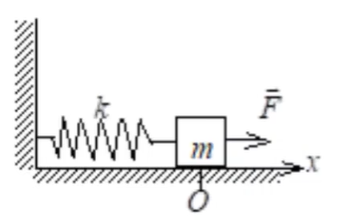
\includegraphics[width=0.25\linewidth]{figures/screenshot003}
		%\caption{}
		\label{fig:screenshot003}
	\end{figure}
	
	\item 子弹水平射入一段固定在弹簧上、质量为 $M$ 的木块内，弹簧劲度系数为 $k$。若测得弹簧压缩最大值为 $x$，木块与水平面间的动摩擦因数为 $\mu$，子弹质量为 $m$，求子弹射入的速度大小。
	
	\begin{figure}[H]
		\centering
		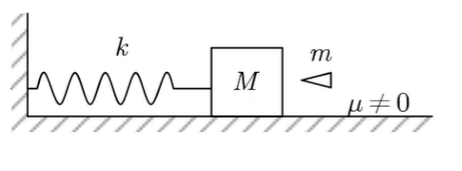
\includegraphics[width=0.35\linewidth]{figures/screenshot005}
		%\caption{}
		\label{fig:screenshot005}
	\end{figure}
	
	

\end{enumerate}

\newpage
\subsection{流体}

\begin{enumerate}
	\item 流体静力学
	\begin{itemize}
		\item 流体静压 $p = p_0 + \rho g h$，液面下深度相同的点压强相等。
		\item 帕斯卡定律：施加于密闭容器内流体的压强将大小不变地传递到流体的各个部分及容器的器壁。
		\item 浮力定律 $F = \rho g V_{\mathrm{排}}$。
		
	\end{itemize}
	
	\item 不可压缩流体的连续性方程
	
	\begin{itemize}
		\item 定常流（稳定流动）：流体的速度仅与位置有关，与时间无关。
		\item 流线：曲线上每一点切线方向与该点流体速度方向一致。
		\item 连续性方程：\(v_1 S_1 = v_2 S_2 = Q\)，其中 \(Q\) 称为流量。
	\end{itemize}
	
	\item 伯努利方程
	
	\begin{itemize}
		\item 若理想流体在重力作用下做定常流，
		\begin{align*}
			\frac{1}{2}\rho v^2 + \rho g h + p = \mathrm{const}.
		\end{align*}
		\item 该方程恒等于单位体积流体所具有的能量。
	\end{itemize}
	
	
\end{enumerate}

\newpage
\subsection{例题5}

\begin{enumerate}
	\item 有一矩形底孔闸门，高 $h=3\,\mathrm{m}$，宽 $b=2\,\mathrm{m}$，上游水深 $h_1=6\,\mathrm{m}$，下游水深 $h_2=5\,\mathrm{m}$。水的密度为 $1.0\times 10^3\,\mathrm{kg/m^3}$，求两侧水作用于闸门上的静压力大小。
	
	\begin{figure}[H]
		\centering
		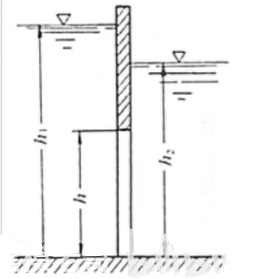
\includegraphics[width=0.35\linewidth]{figures/screenshot006}
		%\caption{}
		\label{fig:screenshot006}
	\end{figure}
	
	\item 水在平管中做定常流，流量为 $4 \times 10^{3}\ \mathrm{cm}^{3}/\mathrm{s}$，粗处截面积为 $40\ \mathrm{cm}^{2}$，细处截面积为 $10\ \mathrm{cm}^{2}$。求水在两处的流速和压强差。
	
	\item 油的密度为 $0.9 \times 10^{3}\ \mathrm{kg}/\mathrm{m}^{3}$，在粗细均匀管道中，$1$ 处比 $2$ 处高 $5.0\ \mathrm{m}$，压强低 $1.2 \times 10^{3}\ \mathrm{Pa}$，求 $5.0\ \mathrm{m}^{3}$ 的油在此过程中的能量损失。
	
	
\end{enumerate}



